 \documentclass{include/protokollclass}
% Main File - Based on protokollclass.cls
% Comments are mostly in English (and some in German, concerning the Praktikum)
% ------------------------------------------------------------------------------
% Further files in folder:
%  - include/cmds.tex (for macros and additional commands)
%  - include/kitlogo.pdf (for titlepage)
%  - lit.bib (bibtex bibliography database)
%  - include/titlepage.tex (for layout of titelpage)
% ------------------------------------------------------------------------------
% Useful Supplied Packages:
% amsmath, amssymb, mathtools, bbm, upgreek, nicefrac,
% siunitx, varioref, booktabs, graphicx, tikz, multicol

\usepackage{rotating}
\usepackage{icomma}
\usepackage{subfig}
\usepackage{pdfpages}
\usepackage[onehalfspacing]{setspace}
\usepackage{lscape} %% Um Tabellen ins Querformat machen zu können



%% ---------------------------------------------
%% |    Informationen über dieses Protokoll    |
%% ---------------------------------------------
\newcommand{\praktikum}{P3}                % P1 oder P2
\newcommand{\semester}{WS17/18}            % z.B. "WS14/15" oder "SS15"

\newcommand{\wochentag}{Mi}                % Mo, Di, Mi oder Do
\newcommand{\gruppennr}{144}                % Zweistellige Gruppennummer

\newcommand{\nachnamea}{Friedrich}             % Nachname des ersten Praktikanten
\newcommand{\vornamea}{Tabea}               % Vorname des ersten Praktikanten
\newcommand{\nachnameb}{Stockmeier}              % Nachname des zweiten Praktikanten
\newcommand{\vornameb}{Lea}              % Vorname des zweiten Praktikanten

\newcommand{\emailadressen}{lea.stockmeier@web.de, tabea.friedrich@t-online.de}
% optionale Angabe von Emailadresse(n) für den Kontakt mit dem Betreuer

\newcommand{\versuch}{Gravimetrie} % Name des Versuchs
\newcommand{\versuchsnr}{00}               % bitte die korrekte Nummer dem 
                                           % Arbeitsplatz am Versuchstag 
                                           % entnehmen
\newcommand{\fehlerrechnung}{Ja}         % Ob Fehlerrechnung im Versuch 
                                           % durchgeführt wurde oder nicht

\newcommand{\betreuer}{Betreuer}      % Name des zuständigen Betreuers
\newcommand{\durchgefuehrt}{00.00.17}      % Datum, an dem der Versuch 
                                           % durchgeführt wurde





%% --------------------------------------
%% |    Settings for Word Separation    |
%% --------------------------------------
% Help for separation:
% In German package the following hints are additionally available:
% "- = Additional separation
% "| = Suppress ligation and possible separation (e.g. Schaf"|fell)
% "~ = Hyphenation without separation (e.g. bergauf und "~ab)
% "= = Hyphenation with separation before and after
% "" = Separation without a hyphenation (e.g. und/""oder)

% Describe separation hints here:
\hyphenation
{
    über-nom-me-nen an-ge-ge-be-nen
    %Pro-to-koll-in-stan-zen
    %Ma-na-ge-ment  Netz-werk-ele-men-ten
    %Netz-werk Netz-werk-re-ser-vie-rung
    %Netz-werk-adap-ter Fein-ju-stier-ung
    %Da-ten-strom-spe-zi-fi-ka-tion Pa-ket-rumpf
    %Kon-troll-in-stanz
}





% um die Titelseite per PDF-reader auszufüllen. Vorgefertigte Daten
% können in Datei 'data.tex' modifiziert werden.
%\setboolean{forminput}{true}
% um die Anmerkungen zu den Textfeldern anzeigen zu lassen
%\setboolean{showannotations}{true}
% Erneuern der Seitenzahl in jedem Kapitel
%\setboolean{chapResetPageNumb}{true}
% Einbinden der Kapitelnummer in der Seitenzahl
%\setboolean{chapWiseNumb}{true}
% english or ngerman (new german für neue deutsche Rechtschreibung statt german)
\SelectLanguage{ngerman}

\title{Geophysikalische Geländeübungen \\ SS 2018 \\ Gravimetrie}
\subtitle{Messgebiet A59/1 (Riedheim)}
\author{\\ Svenja Müller \\ mueller-svenja@gmx.net
\\ \\und\\ \\
Lea Stockmeier \\ lea.stockmeier@web.de \\ \\ \\
Betreuer: Malte Westerhaus und Alexandra Heck}
\date{\vfill\vfill\vfill \today}


%% -----------------------
%% |    Main Document    |
%% -----------------------
\begin{document}
    % Titlepage und ToC
    \FrontMatter
    \maketitle


    \begingroup \let\clearpage\relax    % in order to avoid listoffigures and
    \tableofcontents                    % listoftables on new pages
    \listoffigures
%   \listoftables
    \endgroup
    %\cleardoublepage



    % Contents
    \MainMatter
    
    %\emptychapter[1]{Messprotokoll 1}{} % usage: \emptychapter[page displayed 
                                        %        in toc]{name of the chapter}
    %\pseudochapter[3]{Messprotokoll 2}  % usage: \pseudochapter[number of pages 
                                        %        added]{name of the chapter}
    
 %   \pseudochapter[2]{Versuchsbeschreibung}
%    \pseudochapter[4]{Messprotokoll}

    \chapter{Einleitung}
    Bei der geophysikalischen Geländeübung 2018 führten wir am ersten Messtag, den 22.05., die Magnetik-Messungen durch. Das folgende Protokoll beschreibt die Theorie, Versuchsdurchführung, Auswertung und Fehlerdiskussion zu diesem Versuch.

Bei den Messungen und im Protokoll verfolgten wir folgende Fragestellungen: Die erste große Fragestellung ist, ob mit der Magnetik der Gang lokalisiert werden kann. Bei der Kartierung stellten wir uns die Frage, ob wir den Gang so gut lokalisieren können, dass wir uns daran die Lage der weiteren Profile überlegen können.
Bei den Profilen stellten wir uns dann die Frage, ob diese wirklich senkrecht zum Gang angelegt wurden. Dazu dient vor allem ein Profil, das extra schräg zum Gang gewählt wurde, um zu sehen, ob überhaupt ein Unterschied festgestellt werden kann. Die senkrechten Profile sollen zeigen, ob ein gemeinsames, alle Verläufe der Totalintensitäten erklärendes Modell gefunden werden kann. Die Messungen mit dem Fluxgate verfolgen die Fragestellung, ob dabei sinnvoll das Zweikreisverfahren angewendet werden kann. Die Vermessung eines vorbeifahrenden Traktors und der Umgebung der Basisstation dienten zur Abschätzung der während der Messung durch äußere Einflüsse auftretenden Fehler.

    \chapter{Theoretische Grundlagen}
    \section{kjgkjgr}


    
    \chapter{Versuchsbeschreibung}
    %Versuchsbeschreibung
In der Geoelektrik wurden drei verschiedene Messmethoden verwendet. Das sind die Wenner-Kartierung, Schlumberger-Sondierung und die Tomographie. Sowohl die Wenner-Kartierung als auch die Tomographie wurde über dem Basaltgang durchgeführt, um diese Messmethode mit den übrigen vergleichen zu können.

In Abbildung \ref{abb:PBasalt} sind die Profile der Wenner-Kartierung und Tomographie abgebildet. Die Wenner-Kartierung wurde entlang E11-E12 durchgeführt und das Profil der Tomographie ist in dieser Abbildung beschriftet. Zu sehen ist, dass das Profil der Geoelektrik über dem Profil der Magnetik und Gravimetrie liegt. Dadurch kann man direkt die Messergebnisse vergleichen und eventuell sehen, welche Methode sich zum Untersuchen des Basalts eignet und welche nicht.

Die Schlumberger-Sondierung wurde auf dem gleichen Profil wie die Seismik-Messung mit Sissy durchgeführt, um die beiden Messungen vergleichen zu können. Dieses Profil ist das obere Profil E21-E22 in Abbildung \ref{abb:PWiese}.

%%%%%%%%%%%%%%%%%%%%%%%%%%%%%%%%%%%%%
\begin{figure}[ht]
\centering
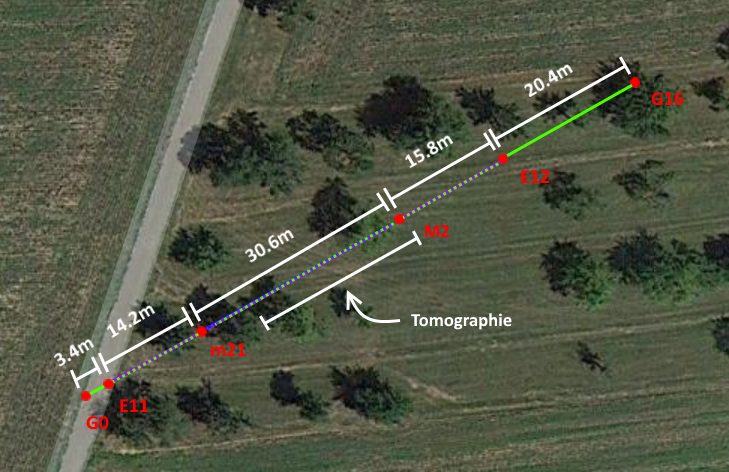
\includegraphics[width=0.6\textwidth]{fig/ElektrikMagnetikGravimetrie0gps.png}
\caption[Profile der Geoelektrik, Gravimetrie und Magnetik des Messgebiets am Basaltgang]{Profile der Geoelektrik, Gravimetrie und Magnetik des Messgebiets am Basaltgang. Die Graphik wurde von Rebekka Kirchgässner und Luisa Rank übernommen.}
\label{abb:PBasalt}
\end{figure}
%%%%%%%%%%%%%%%%%%%%%%%%%%%%%%%%%%%%

%%%%%%%%%%%%%%%%%%%%%%%%%%%%%%%%%%%%%
\begin{figure}[ht]
\centering
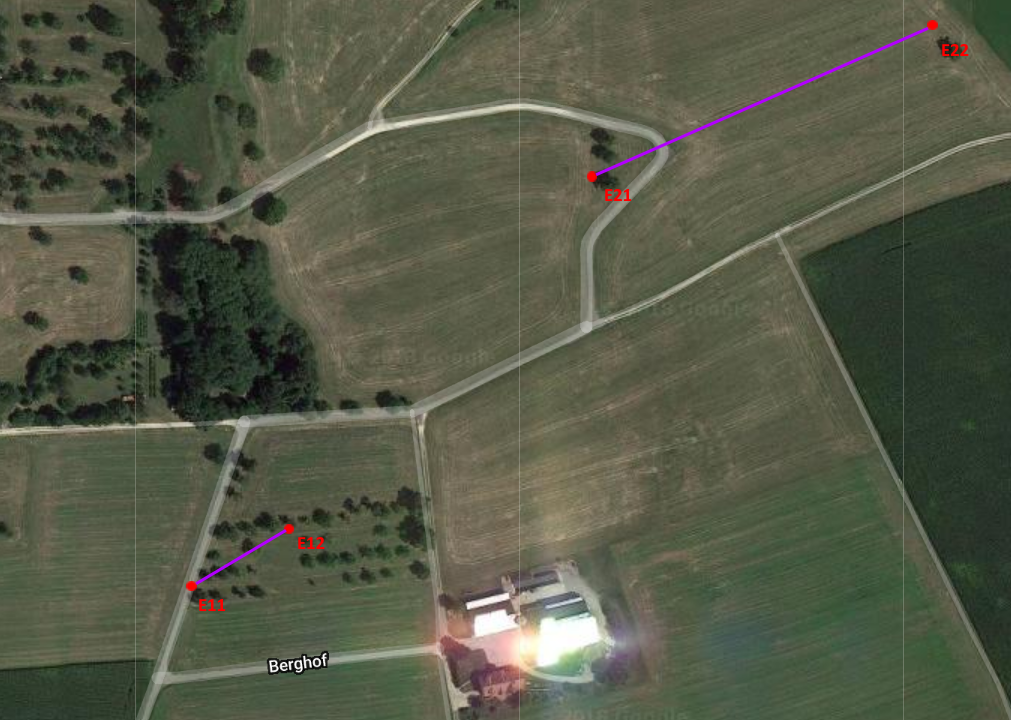
\includegraphics[width=0.6\textwidth]{fig/profilegps.PNG}
\caption[Profil E11-E12 und E21-E22 auf den beiden Messgebieten]{Profil E11-E12 und E21-E22 auf den beiden Messgebieten. Die Graphik wurde von Rebekka Kirchgässner und Luisa Rank übernommen.}
\label{abb:PWiese}
\end{figure}
%%%%%%%%%%%%%%%%%%%%%%%%%%%%%%%%%%%%
\newpage

\section{Wenner-Katierung}

Begonnen wurde mit der Wenner-Kartierung, um die Lage des Basaltgangs genauer zu bestimmen. Damit wir die Tomographie möglichst genau über dem Gang durchführen
können. 
Des weiteren soll eingeschätzt werden, wie gut diese Methode zum Vermessen des Basaltgangs geeignet ist.

Die Kartierung wurde in einer Tiefe von 5\,m vorgenommen. Dies ist begründet mit der Annahme, dass der Basaltgang vermutlich in ca. 1-2\,m Tiefe beginnt und nach unten 
als unendlich angenommen werden kann. Je mehr Basalt im Bereich der Messung ist, desto größer ist die Auswirkung auf die Ergebnisse.
Die Anordnung ist orthogonal zum Basaltgang und wird auch orthogonal dazu verschoben. Orientiert wurde sich dabei an der Messung von Magnetik, es wurde 
entlang des Magnetik-Profils M2-M21 gemessen. Dabei wurde darauf geachtet, dass auch eine Messung komplett außerhalb 
des Einflussbereichs des Basalt liegt.

\section{Tomographie}

Die Tomographie ist eine Kombination der ersten beiden Messmethoden. Sie wurde auf dem gleichen Profil wie die Wenner-Kartierung durchgeführt.
Es wurden 48 Elektroden verwendet, die in einem Abstand von 50\,cm, auf der gleichen Messlinie wie bei der Wenner-Kartierung aufgestellt waren. 
Die Mitte der Messlinie wurde auf einen Punkt gesetzt, an dem auch die Mitte des Basaltgangs vermutet wurde. Insgesamt wurde also auf einer Länge von 24\,m gemessen.
Als 0-Punkt für die Messung wurde das obere Ende des Messbands festgelegt.
Nachdem die Elektroden aufgestellt und angeschlossen wurden, wurde die Messung automatisch mit einem Messgerät ausgeführt. Auf das Ergebnis musste ungefähr 
eine Stunde gewartet werden. Das Messprotokoll zur Tomographie befindet sich im Anhang unter der Abbildung \ref{abb:AnhTomographie}.

\section{Schlumberger-Sondierung}

Sie Schlumberger-Sondierung wurde nicht auf dem Messgebiet über dem Basaltgang vorgenommen, sondern auf einer Wiese wesentlich weiter oben. Auf dieser Wiese wurde 
bereits mit der Seismik gemessen. Um unsere Ergebnisse von der Seismik-Messung und dieser Messung vergleichen zu können, wurde die Messung entlang der gleichen
Linie durchgeführt.

Da wir kein sehr großes, gerades Gelände hatten und auch mit der Seismik in keinen großen Tiefen gemessen wurde, betrug die Länge des Profils 200\,m. Als Mitte 
haben wir den Punkt des Mittelschusses der Hammerschlag-Methode (Seismik) verwendet.
In der Mitte des Profils haben wir angefangen, die Elektroden zu stecken. In beide Richtungen haben wir den Abstand exponentiell vergrößert. Die genauen Abstände kann man dem Messprotokoll dieser Messung im Anhang entnehmen.
    
    \chapter{Auswertung}
    \section{Kalibrierung des Torsions-Magnetometers}

Die Messwerte der Kalibrierungsmessung sind in Abbildung \ref{fig:MPKalibrierung} zu sehen. Zur Auswertung wird zunächst der durch die Spulen fließende Strom mit dem Spulenkennwert $s$ und der Formel
\begin{equation}
 B=s\cdot I=I\cdot \eb{26,5}{nT}{mA} 
\end{equation}
in das Magnetfeld umgerechnet. Der Plot der Messwerte und der linearen Regression ist in Abbildung \ref{fig:kalibrierung} zu sehen. Bei der Regression ergab sich eine Steigung von $\eb{-0.0039}{Skt}{nT}$. Der negative Kehrwert dieser Steigung liefert den Kalibrierungsfaktor
\begin{equation}
 \frac{\tau}{|\vec{m}|}=\eb{253}{nT}{Skt} \fullstop
\end{equation}

\begin{figure}
 \centering
 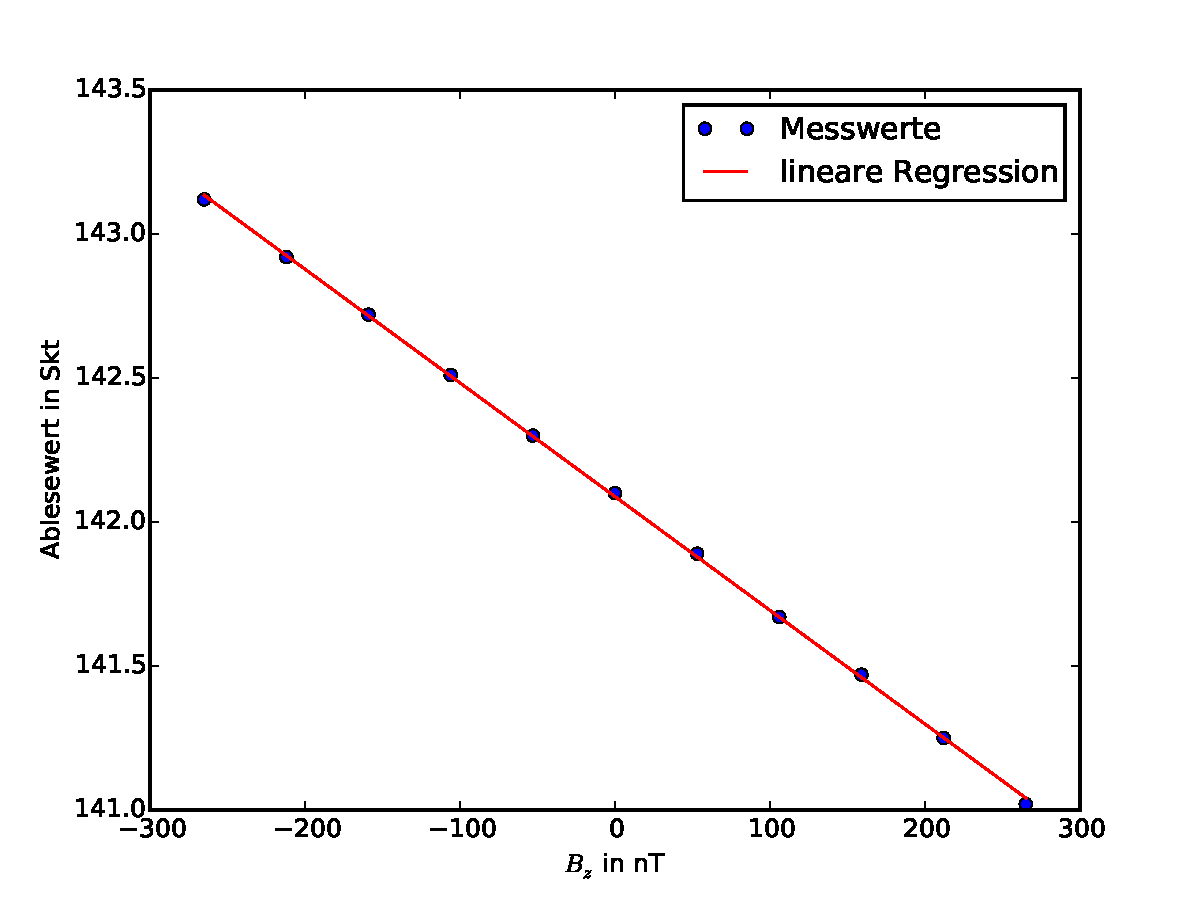
\includegraphics[width=\textwidth]{fig/kalibrierung.pdf}
 \caption[Bestimmung des Kalibrierungsfaktors des Torsions-Magnetometers]{Bestimmung des Kalibrierungsfaktors des Torsions-Magnetometers. Aufgetragen sind die Ablesewerte am Gfz in Skt über die angelegte magnetische Flussdichte in nT}
 \label{fig:kalibrierung}
\end{figure}


% \begin{figure}
%  \centering
%  \includegraphics[width=\textwidth]{fig/}
%  \caption{}
%  \label{fig:}
% \end{figure}
    
    \chapter{Fehlerbetrachtungen}
    \section{Einfluss äußerer Störfaktoren auf die Basisstation}

Um eine Einschätzung dafür zu bekommen, wie sehr das Magnetfeld an der Basisstation von äußeren Störfaktoren, wie zum Beispiel der Hütte, abhängig war, wurde ein Profil von der Basisstation aus an der Hütte vorbei gelegt. Das zugehörige Messprotokoll befindet sich im Anhang in Abbildung \ref{fig:MPHuette}.


In Diagramm \ref{fig:plot_huette} sind die Messergebnisse graphisch dargestellt. Es ist zu erkennen, dass das Magnetfeld bei 19\,m, also neben der Hütte, abnimmt. In der Nähe der Basisstation wird der Messwert jedoch wieder annähernd konstant. Um jedoch sicher sagen zu können, dass der Einfluss der Hütte nur bis zu einer Entfernung von 5\,m zu messen ist, hätten wir die Messung auf der anderen Seite der Basisstation noch weiter führen müssen.

\begin{figure}[!ht]
 \centering
 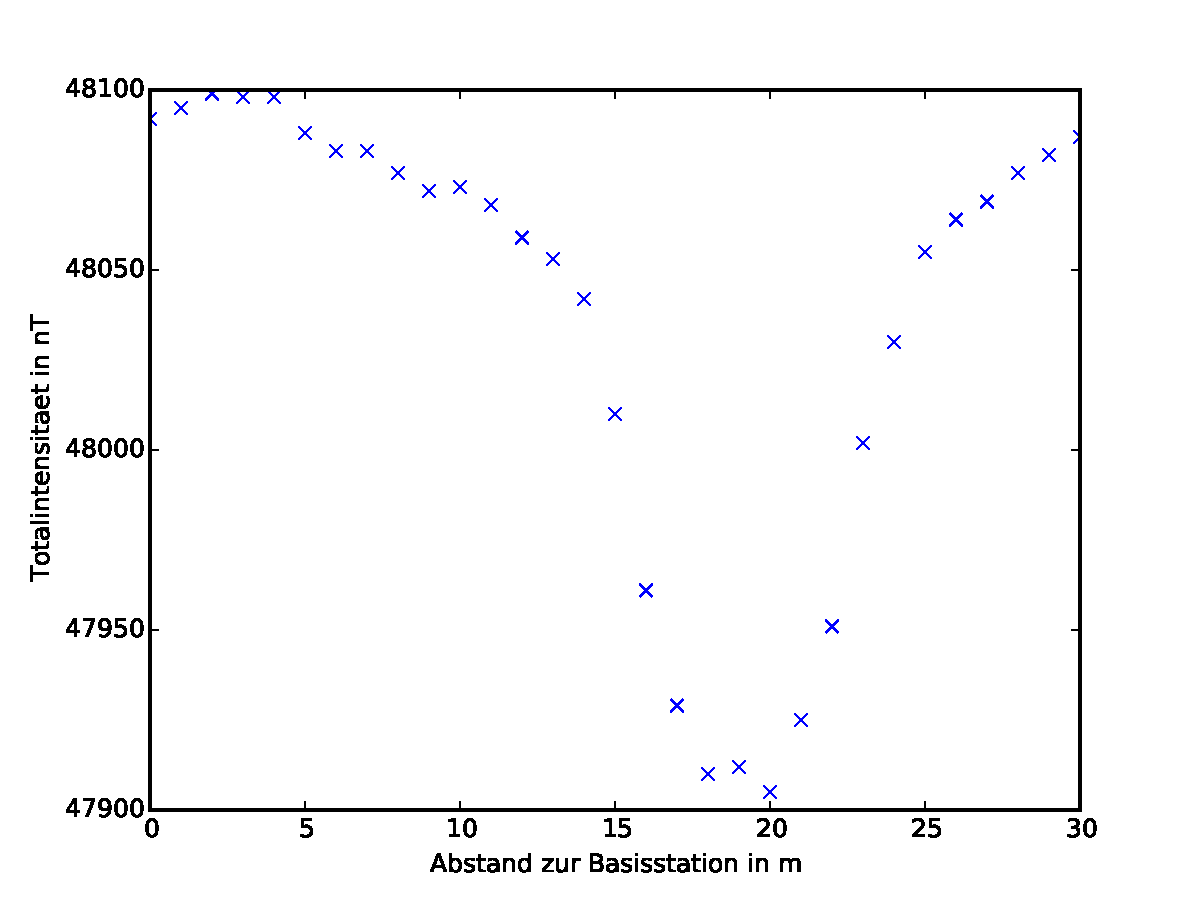
\includegraphics[width=\textwidth]{fig/plot_huette.pdf}

In Diagramm \ref{fig:plot_huette} sind die Messergebnisse graphisch dargestellt. Es ist zu erkennen, dass das Magnetfeld bei 19\,m, also neben der Hütte, abnimmt. In der Nähe der Basisstation wird der Messwert jedoch wieder annähernd konstant. Um jedoch sicher sagen zu können, dass der Einfluss der Hütte nur bis zu einer Entfernung von 5\,m zur Basisstation zu messen ist, hätten wir die Messung auf der anderen Seite der Basisstation noch weiter führen müssen.

\begin{figure}[!ht]
 \centering
 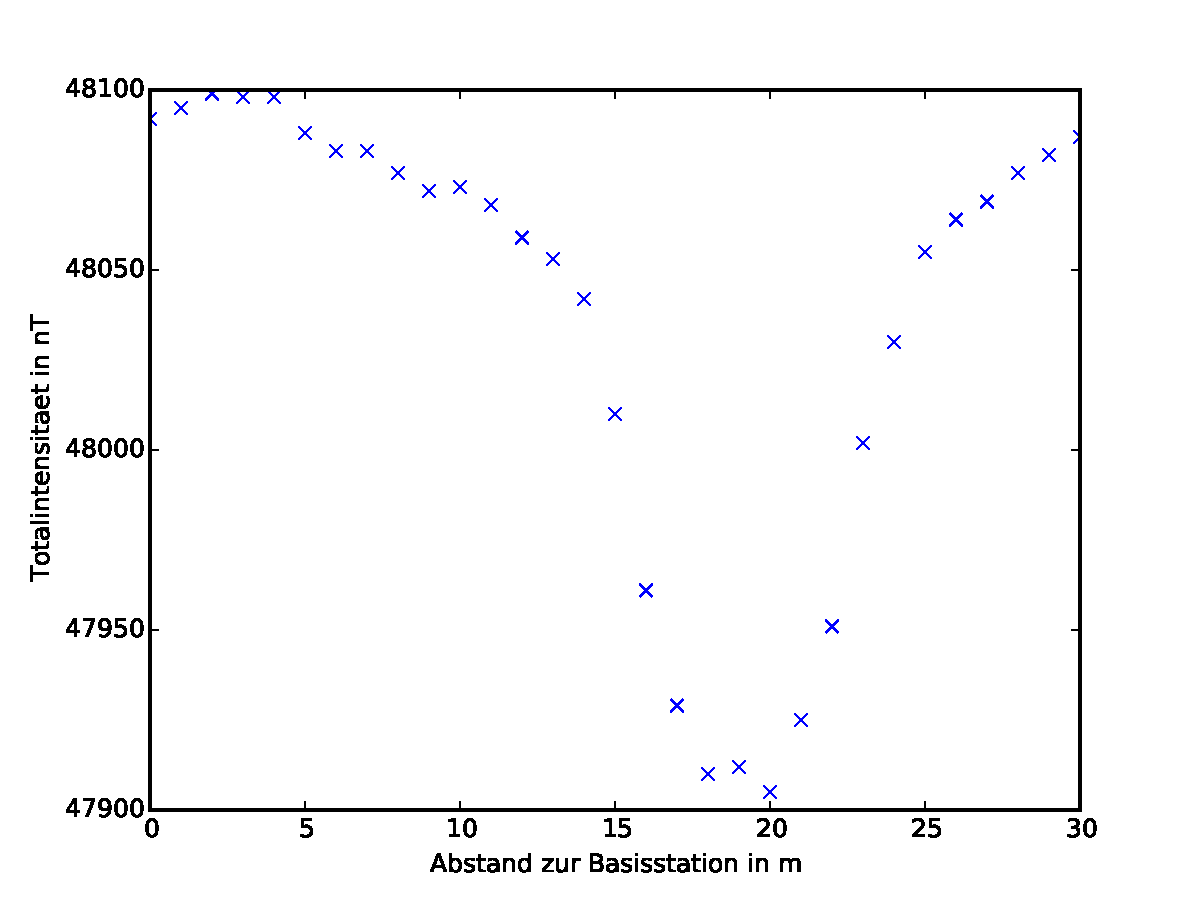
\includegraphics[width=0.7\textwidth]{fig/plot_huette.pdf}

 \caption[Einfluss der Umgebung auf die Basismessung]{Einfluss der Umgebung auf die Basismessung. Die Totalintensität in nT ist über dem Abstand zur Basisstation in m aufgetragen. Der Tisch mit vielen Arbeitsmaterialien befindet sich bei 13,5\,m und die Hütte bei 19\,m.}
 \label{fig:plot_huette}
\end{figure}


% \begin{figure}[h!]

% \begin{figure}[!ht]

%  \centering
%  \includegraphics[width=\textwidth]{fig/Messprotokolle/}
%  \caption{}
%  \label{fig:}
% \end{figure}

\section{Einfluss eines vorbeifahrenden Traktors}

Es fuhr an diesem Tag mehrmals ein kleiner Traktor an der Messwiese vorbei. Um seinen Einfluss auf das lokale Magnetfels zu untersuchen, wurde während einer Vorbeifahrt eine Messung mit dem Gradiometer durchgeführt. Dieses wurde in einem Abstand von circa einem Meter neben dem Feldweg möglichst still gehalten. Das Diagramm dieser Messung ist in Abbildung \ref{fig:plot_traktor} zu sehen.

\begin{figure}[!ht]
 \centering

 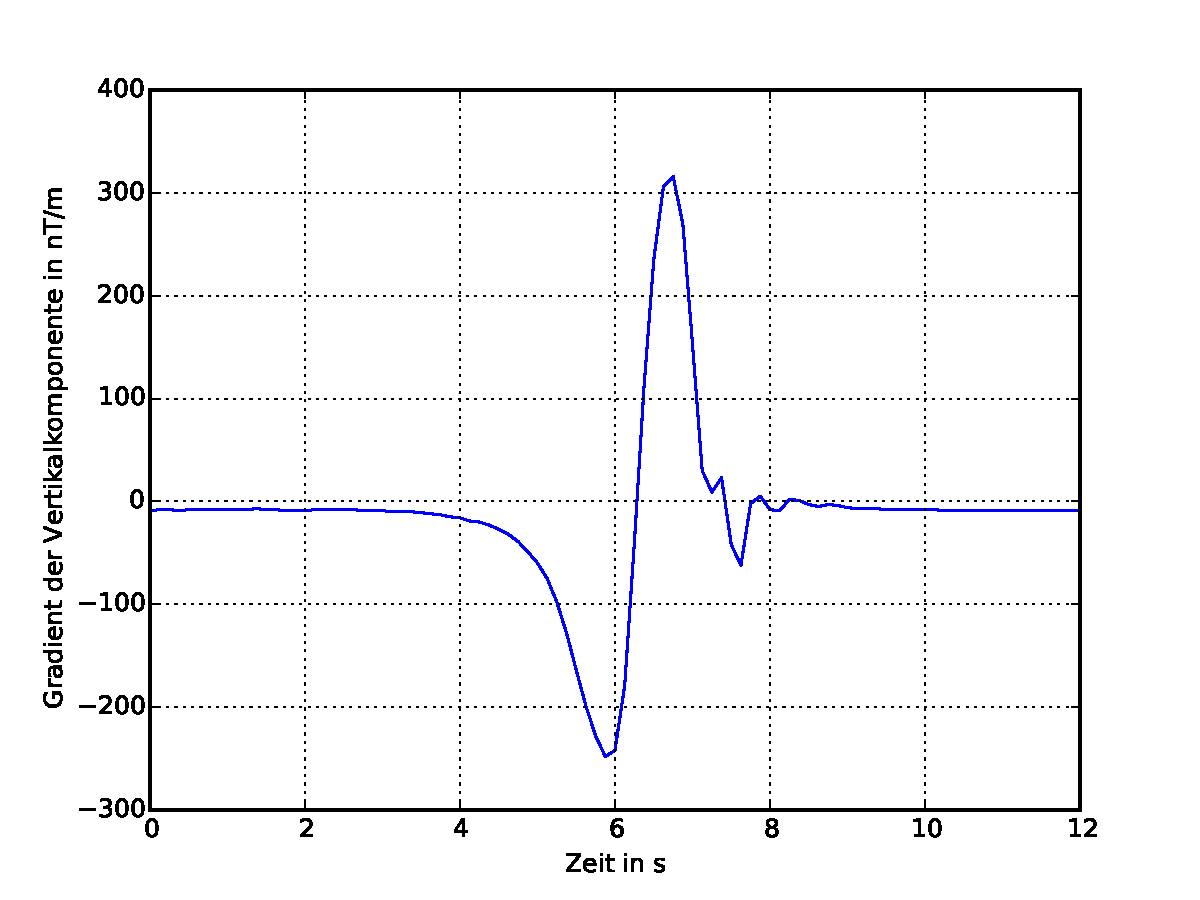
\includegraphics[width=\textwidth]{fig/traktor_ausschnitt.pdf}

 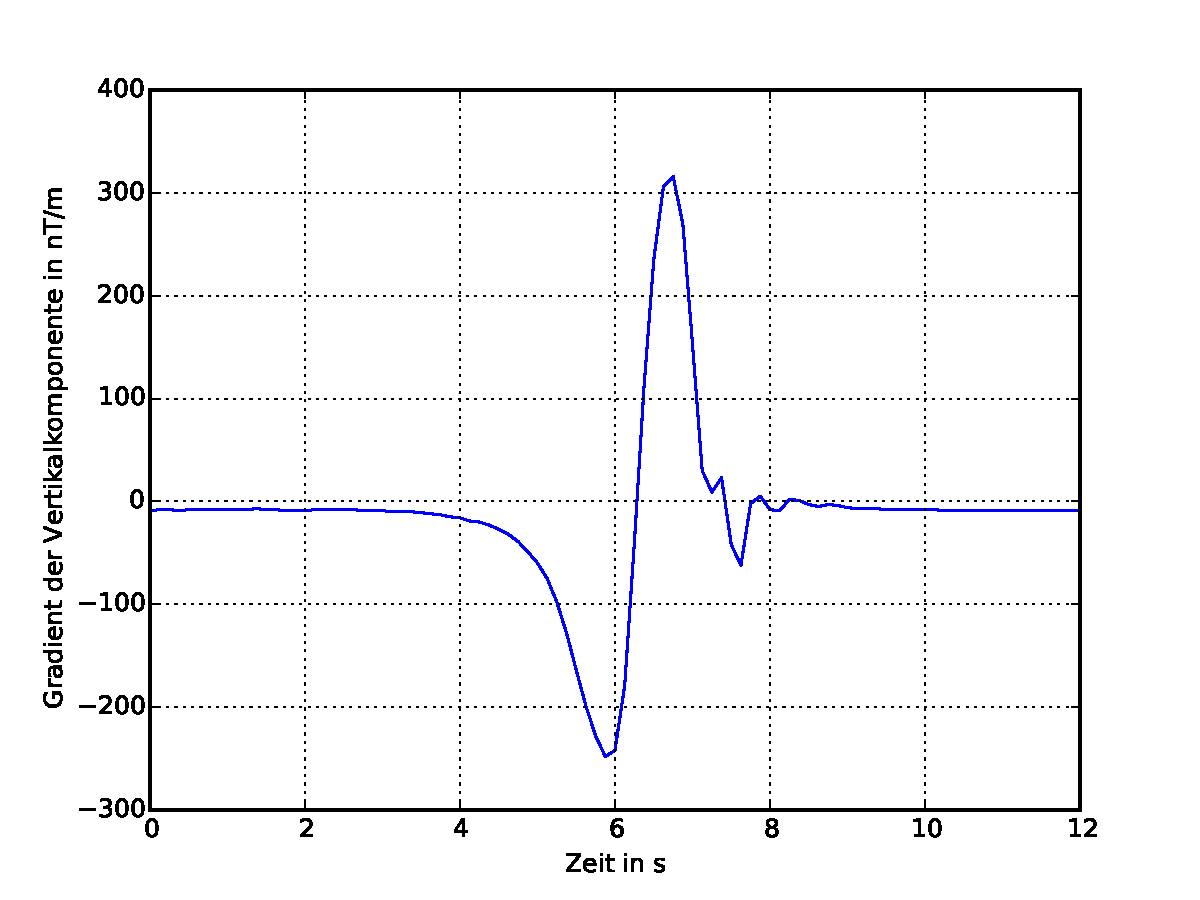
\includegraphics[width=0.7\textwidth]{fig/traktor_ausschnitt.pdf}

 \caption[Messung während einer Vorbeifahrt des Traktors]{Messung während einer Vorbeifahrt des Traktors. Der Gradient der Vertikalkomponente ist über der Zeit nach Beginn der Messung aufgetragen. Es wurde 30\,s lang gemessen. Da der Einfluss nur bis zu Sekunde 9 zu sehen ist, ist hier nur der entsprechende Ausschnitt gezeigt.}
 \label{fig:plot_traktor}
\end{figure}


Zur Zeit der Peaks war der Traktor dem Gradiometer am nächsten. Es ist also deutlich zu erkennen, dass der Traktor einen Einfluss auf das Magnetfeld seiner Umgebung hat. Es ist außerdem zu erkennen, dass der Einfluss sechs Sekunden lang in Form mehrerer Ausschläge zu messen war. Unter der Annahme, dass dieser mit einer Geschwindigkeit von $\eb{20}{km}{h}\approx\eb{5,6}{m}{s}$ fuhr, ist sein Einfluss mit dem Gradiometer also in einer Distanz von $\eb{5,6}{m}{s}\cdot\e{3}{s}\approx\e{16,7}{m}$ noch zu messen. Damit ist sein Einfluss größer als erwartet und es hätte noch genauer darauf geachtet werden müssen, nicht bei einer Vorbeifahrt zu messen.
Zur Zeit der Peaks war der Traktor dem Gradiometer am nächsten. Es ist also deutlich zu erkennen, dass der Traktor einen Einfluss auf das Magnetfeld seiner Umgebung hat. Es ist außerdem zu erkennen, dass der Einfluss sechs Sekunden lang in Form mehrerer Ausschläge zu messen war. Unter der Annahme, dass dieser mit einer Geschwindigkeit von $\eb{20}{km}{h}\approx\eb{5,6}{m}{s}$ fuhr, ist sein Einfluss mit dem Gradiometer also in einer Distanz von $\eb{5,6}{m}{s}\cdot\e{3}{s}\approx\e{16,7}{m}$ noch zu messen. Damit ist sein Einfluss größer als erwartet und es hätte noch genauer darauf geachtet werden müssen, nicht bei einer Vorbeifahrt zu messen. Auf die Basisstation hatte er aber vermutlich keinen Einfluss mehr, weil er sich nie näher als circa 60\,m von der Basisstation entfernt befand.



    \chapter{Zusammenfassung}
    Insgesamt bewerten wir die aus den Magnetik-Messungen gewonnenen Ergebnisse als sehr gut. Dies liegt besonders daran, dass auf den Ergebnissen der Magnetik-Kartierung die gesamten weiteren Planungen der Messungen während der Messwoche aufbauten. Dadurch lagen unsere Profile senkrecht zum Gang, was für die Magnetik-Auswertung von großer Bedeutung war. Für die Gravimetrie reichte es, den Winkel zur Streichrichtung des Gang zu kennen, was durch die senkrechte Lage auch gegeben war.

Die Fragestellung nach der Lokalisierung des Gangs kann bejaht werden, da dieser mit der Kartierung eindeutig lokalisiert werden konnte. Die Lokalisierung reichte auch aus, um die Lage der Profile festzulegen. Auch das extra schräg zum Gang angeordnete Profil erfüllte seinen Zweck und zeigte uns, dass eine schräge Lage zum Gang einen sehr viel breiteren Verlauf des Maximums zur Folge hat.

Für die drei nah aneinander liegenden Profile konnte ein Modell gefunden werden, das den Verlauf der Totalintensität über allen drei Profilen erklärt. Die Richtigkeit dieses Modell ist jedoch nur schwer zu überprüfen, weil bei der Modellierung viele Annahmen getroffen werden mussten. Es ergibt sich jedoch bei Profil M21-M2 eine Breite von $\e{(4,4\pm0,5)}{m}$ bei einem Neigungswinkel von $(16\pm3)^\circ$ gemessen von der senkrechten aus in Richtung Ost. Die Tiefe der Gangoberkante bei diesem Profil als $\e{(1,6\pm0,5)}{m}$ bestimmt werden.

Diese Ergebnisse können gut mit denen der Gravimetrie verglichen werden, weil die Gravimetrie-Messung auch entlang des Profils M21-M2 durchgeführt wurde. Es ergab sich, je nach Modell, eine Breite von $\e{(4,41\pm0,40)}{m}$ bzw. $\e{(4,54\pm0,58)}{m}$. Alle drei Breiten liegen in den Fehlergrenzen der jeweils anderen Messungen. Die Vergleichbarkeit ist dennoch nicht wirklich gut gegeben, weil die Tiefe der Gangoberkante und der Neigungswinkel bei den Gravimetrie-Modellierungen ganz andere Werte ergaben. Die Tiefe wurde als $\e{(0,397\pm0,010)}{m}$ bzw. 1,5\,m modelliert und der Neigungswinkel war $30^\circ$ bzw. $0^\circ$.

Die Fluxgate-Messungen zeigten, dass das Zweikreisverfahren für unsere Messungen nicht angewendet werden kann und die Vermessung eines Traktors und der Umgebung der Basisstation halfen bei der Einschätzung der während der Messungen gemachten Fehler.

    % appendix for more or less interesting calculations
   \Appendix
   \chapter*{\appendixname} \addcontentsline{toc}{chapter}{\appendixname}
    % to make the appendix appear in ToC without number. \appendixname = 
    % Appendix or Anhang (depending on chosen language)
    \section{Messprotokolle}

\begin{figure}[h!]
 \centering
 \includegraphics[width=0.8\textwidth]{fig/Messprotokolle/Kalibrierung.png}
 \caption{Messprotokoll zur Kalibrierungsmessung}
 \label{fig:MPKalibrierung}
\end{figure}

\begin{figure}[h!]
 \centering
 \includegraphics[width=\textwidth]{fig/Messprotokolle/EinflussHuette.png}
 \caption{Messprotokoll zum Profil zur Untersuchung der Einflüsse äußerer Störfaktoren auf die Basismessung}
 \label{fig:MPHuette}
\end{figure}

% \begin{figure}[h!]
%  \centering
%  \includegraphics[width=\textwidth]{fig/Messprotokolle/}
%  \caption{}
%  \label{fig:}
% \end{figure} %\cleardoublepage



    % Bibliography
    \TheBibliography

    % BIBTEX
    % use if you want citations to appear even if they are not referenced to: 
    % \nocite{*} or maybe \nocite{Kon64,And59} for specific entries
    %\nocite{*}
    \bibliographystyle{babalpha}
    \bibliography{lit.bib}

    % THEBIBLIOGRAPHY
    %\begin{thebibliography}{000}
    %    \bibitem{ident}Entry into Bibliography.
    %\end{thebibliography}
\end{document}
